\documentclass[10pt,a4paper]{article}
\usepackage[margin=2.1cm]{geometry}
\usepackage{amsmath,amssymb,graphicx,booktabs,caption,float,xcolor,enumitem}
\usepackage{tikz,array}
\usetikzlibrary{arrows.meta,positioning}
\usepackage[colorlinks=true,linkcolor=blue!50!black,citecolor=blue!50!black,urlcolor=blue!50!black]{hyperref}
\captionsetup{font=small,labelfont=bf}
\setlist{itemsep=1pt,topsep=3pt}
\graphicspath{{figures/}}
\definecolor{cA}{HTML}{3b75af}
\definecolor{cC}{HTML}{d1495b}
\newtheorem{result}{Result}

\title{\textbf{Fact flow, finite copies and susceptibility:}\\[2pt]
\textbf{a minimal theory of the reading reversal and of persistence}}
\author{Claude (theory work, \nolinkurl{analysis/theory_claude/}), in exchange with the ChatGPT agent}
\date{Session report, 27--28 October 2026}

\begin{document}
\maketitle

\begin{abstract}
\noindent
We look for the smallest model that \emph{explains} two phenomena of swarms of Bayesian agents under a covert controller.
The \emph{reading reversal}: reading more helps the controller when memory is short and protects the swarm when memory
is long. \emph{Persistence}: the controller's effect outlasts its posting in one task (task003) but fades in another
(Object Placements, OP). Our aim is understanding, not numerical agreement with the simulator; none of the models below
calls the Bayesian engine or uses a task world. Four findings.
\begin{enumerate}
\item A two-class \emph{fact-flow} model, in which facts move between memories and a board and agents vote through a
  sigmoid, shows the reversal for parameters fixed in advance. It explains it as \emph{evidence displacement against
  sensitivity}, with no proof needed.
\item Making the same model finite, so that facts can die out, raises the controller's effect fourfold, to the
  simulator's level. The reason is that the swarm's spread-out evidence \emph{collapses} while the controller's few facts
  survive. The relevant finite size is copies per fact. Tying reposting to the vote turns flat persistence into slow
  fading.
\item The agents' own counter-evidence strength, measured from stored memories, orders the four setups' crossovers.
  Completed proofs are too rare at the crossover to matter.
\item The persuasiveness of a controller fact depends on which fact it is and on the receiver's context. The population's
  \emph{susceptibility} to the controller facts it actually encounters falls where persistence fades and stays flat where
  it persists.
\end{enumerate}
We also describe the ChatGPT agent's independent model, which explains the reversal by reading completing an
all-or-nothing correction, and compare it with ours. The two agents converged on a common model with three layers:
circulation with a growth threshold and irreversible loss of diversity, a sigmoid response to net evidence, and at most
one context variable. What remains open is a compact law for how susceptibility evolves.
\end{abstract}

% ======================================================================================================================
\section{Introduction}
The simulator is a swarm of $N=24$ exact Bayesian agents. They read a shared board, forget facts at rate
$\gamma=-\ln\rho$, vote, and repost. A covert controller posts true facts selected to push a wrong answer $A2$ until
$T=30$. The controller effect $G$ is the difference in the share of $A2$ votes between a controlled and a silent run; the
reading increment is $D(q_1\!\to\!q_2)=G(q_2)-G(q_1)$; and $\delta(t)$ is the effect after the stop. Two phenomena hold
in both tasks (task003 and MuSR Object Placements) and both setups (\emph{symmetric}: the agents can jointly prove the
right answer; \emph{no-proof}: they cannot):
\begin{itemize}
\item[(I)] \textbf{reading reversal:} $D>0$ at short memory and $D<0$ at long memory, with a crossover that moves to
  shorter memory as $q$ grows;
\item[(II)] \textbf{persistence:} after the stop, $\delta$ stays nearly flat in task003 but fades by 30--60\% in Object
  Placements. A frozen board keeps it, and no communication removes it.
\end{itemize}
Earlier models reproduced these numerically but kept the exact Bayesian engine inside, so they could not say
\emph{why}. This session followed the researcher's plan of 27 October: build the smallest engine-free dynamics, judged
on whether it shows both phenomena and on whether we can explain them. Every test below had its expectation written down
before running. Failures are reported alongside successes.

% ======================================================================================================================
\section{A minimal fact-flow model}
\begin{figure}[h]
\centering
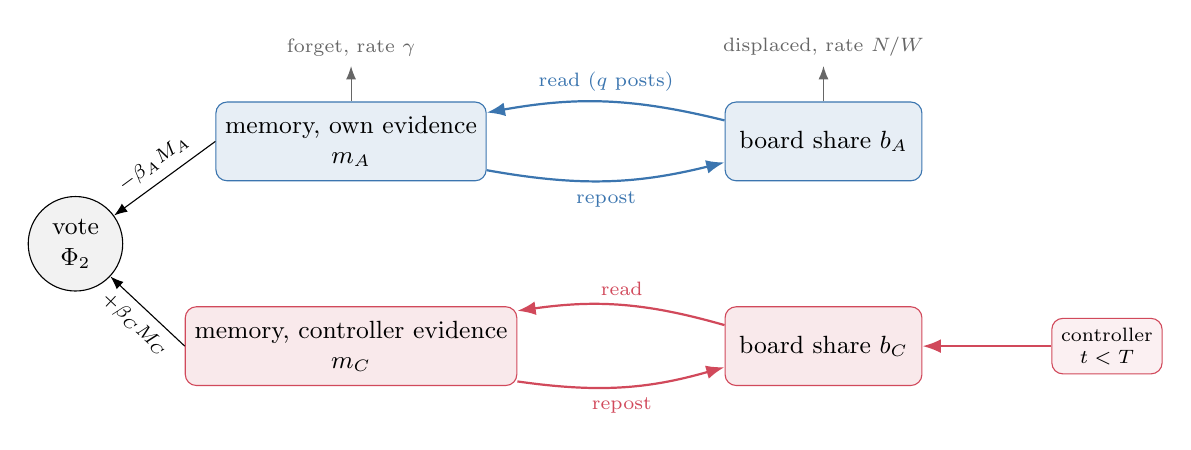
\begin{tikzpicture}[font=\small, >=Latex,
  res/.style={draw, rounded corners, minimum width=25mm, minimum height=10mm, align=center},
  lab/.style={font=\scriptsize, align=center}]
  \node[res, fill=cA!12, draw=cA] (mA) at (0,1.3) {memory, own evidence\\ $m_A$};
  \node[res, fill=cC!12, draw=cC] (mC) at (0,-1.3) {memory, controller evidence\\ $m_C$};
  \node[res, fill=cA!12, draw=cA] (bA) at (6.0,1.3) {board share $b_A$};
  \node[res, fill=cC!12, draw=cC] (bC) at (6.0,-1.3) {board share $b_C$};
  \node[draw, circle, fill=black!5, minimum size=12mm, align=center] (V) at (-3.5,0) {vote\\ $\Phi_2$};
  \node[draw=cC, rounded corners, fill=cC!8, font=\scriptsize, align=center] (ctrl) at (9.6,-1.3) {controller\\ $t<T$};
  \draw[->, thick, cA] (bA) to[bend right=12] node[lab, above] {read ($q$ posts)} (mA);
  \draw[->, thick, cA] (mA) to[bend right=12] node[lab, below] {repost} (bA);
  \draw[->, thick, cC] (bC) to[bend right=12] node[lab, above] {read} (mC);
  \draw[->, thick, cC] (mC) to[bend right=12] node[lab, below] {repost} (bC);
  \draw[->, thick, cC] (ctrl) -- (bC);
  \draw[->] (mA.west) -- node[lab, above, sloped] {$-\beta_A M_A$} (V);
  \draw[->] (mC.west) -- node[lab, below, sloped] {$+\beta_C M_C$} (V);
  \draw[->, black!60] (mA.north) -- ++(0,0.45) node[lab, above] {forget, rate $\gamma$};
  \draw[->, black!60] (bA.north) -- ++(0,0.45) node[lab, above] {displaced, rate $N/W$};
\end{tikzpicture}
\caption{\textbf{The fact-flow model.} Facts of two classes, the agents' own (A) and the controller's (C), circulate
between agents' memories and the board. The vote depends on how much of each an agent holds, and the vote can in turn
gate what is reposted.}
\label{fig:model}
\end{figure}

Each class $\alpha\in\{A,C\}$ has $F_\alpha$ interchangeable facts. Let $m_\alpha$ be the chance that an agent holds a
given class-$\alpha$ fact, $M_\alpha=F_\alpha m_\alpha$ the number it holds, and $b_\alpha$ the class's share of the board
(Fig.~\ref{fig:model}). Agents act at rate 1 and read $q$ of the $W=48$ newest posts. The board turns over at rate $N/W$.
The controller posts at rate $\lambda_0$ until $T$:
\begin{align}
\dot m_\alpha&=(1-m_\alpha)\,r_\alpha-\gamma m_\alpha,\qquad r_\alpha=1-(1-b_\alpha/F_\alpha)^q,\label{eq:m}\\
\dot b_\alpha&=\tfrac NW(S_\alpha-b_\alpha)+\tfrac{\lambda(t)}W(u_\alpha-b_\alpha),\qquad u_C=1,\ u_A=0,\label{eq:b}\\
\Phi_2&=\sigma(x),\qquad x=h_0+\beta_C M_C-\beta_A M_A,\label{eq:phi}\\
S_\alpha&\propto\kappa_\alpha M_\alpha\,g_\alpha,\qquad g_C=\varepsilon+(1-\varepsilon)\Phi_2,\quad g_A=\varepsilon+(1-\varepsilon)(1-\Phi_2),\label{eq:S}
\end{align}
with a background weight $\kappa_0$, which represents a neutral third kind of post. The gating parameter $\varepsilon$
sets how much reposting depends on the vote: $\varepsilon=1$ is neutral, $\varepsilon=0$ means only $A2$ voters repost
controller facts. Parameters were fixed before any run: $N/W=0.5$, $F_A=16$, $F_C=4$, $\beta_A=\beta_C=0.5$,
$h_0=\ln\tfrac12$, $\kappa_A=\kappa_C=1$, $\kappa_0=0.2$, $\lambda_0=1$. The controlled arm has $\lambda_0>0$, the silent
arm none.

% ======================================================================================================================
\section{The reading reversal: displacement against sensitivity}
\begin{figure}[h]
\centering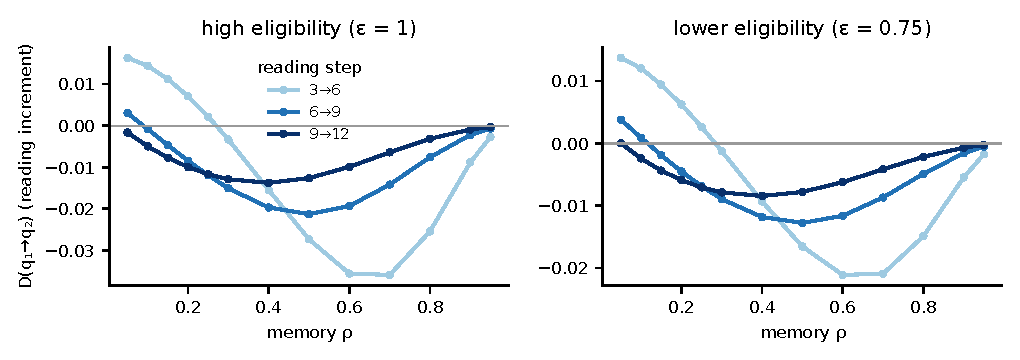
\includegraphics[width=\linewidth]{fig2_mf_reversal.pdf}
\caption{\textbf{The reversal in the mean-field model} for two gatings. The crossover moves to shorter memory as $q$
grows, as in the simulator.}
\label{fig:mfrev}
\end{figure}
The model shows the reversal for the parameters fixed in advance (Fig.~\ref{fig:mfrev}): $D(3\to6)=+0.003$ at
$\rho=0.05$ and $-0.005$ at $\rho=0.5$. The crossover lies between 0.2 and 0.3 for $3\to6$, between 0.1 and 0.2 for
$6\to9$, and between 0.05 and 0.1 for $9\to12$. The reversal holds in 16 of 22 single-parameter changes. It needs
\emph{no} proof, \emph{no} selective reposting, and \emph{no} concentration of controller facts (it survives
$F_C=F_A$). That last point refuted the mechanism I had predicted in advance.

\paragraph{Mechanism.} Let $x_s$ be the silent arm's operating point and
$B=\beta_C M_C-\beta_A(M_A^{C}-M_A^{S})$ the controller's \emph{net} evidence displacement. $B$ includes the agents'
own evidence that the controller crowds out (a correction by the ChatGPT agent). Then exactly
$G=\sigma(x_s+B)-\sigma(x_s)$, and
\begin{equation}
\partial_q G=\sigma'(x_c)\,\partial_q B+\beta_A\,\partial_q M_A^{S}\,\big[\sigma'(x_s)-\sigma'(x_c)\big].\label{eq:rev}
\end{equation}
The first term is exposure: reading spreads the controller's displacement. The second is \emph{sensitivity}: reading
also accumulates the agents' own evidence, which moves the population away from the tipping point, where the sigmoid is
flatter. With short memory, little own evidence accumulates and exposure wins; with long memory, the sensitivity loss
wins (Fig.~\ref{fig:dose}).
\begin{figure}[h]
\centering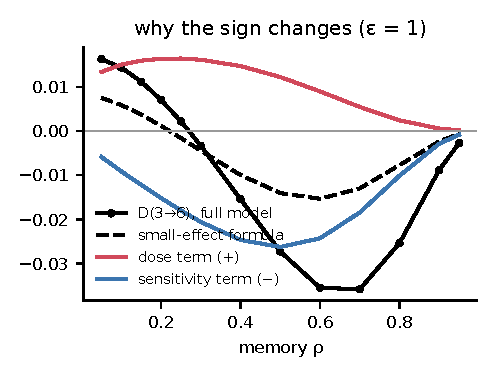
\includegraphics[width=0.48\linewidth]{fig3_dose_sensitivity.pdf}
\caption{\textbf{Why the sign changes:} the reading increment of the full model, a small-effect formula, and its two
competing terms.}
\label{fig:dose}
\end{figure}

% ======================================================================================================================
\section{Persistence in the mean field: a growth threshold}
Linearising Eqs.~\eqref{eq:m}--\eqref{eq:b} for rare controller facts after the stop gives a growth threshold:
\begin{equation}
\mathcal R_C=\frac{q\,\kappa_C\,g_C}{\gamma\,H}>1,\qquad H=\kappa_A M_A g_A+\kappa_0.\label{eq:R}
\end{equation}
Controller facts keep circulating after the stop if and only if $\mathcal R_C>1$; the board's turnover sets the speed,
not the threshold. Fig.~\ref{fig:thr} shows that the retained effect is about zero below the threshold and rises above
it.
\begin{figure}[h]
\centering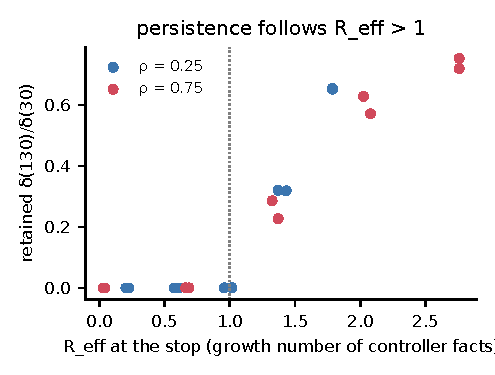
\includegraphics[width=0.46\linewidth]{fig4_threshold.pdf}
\caption{\textbf{Retained effect against the growth number} $\mathcal R_C$ (mean field, all gatings).}
\label{fig:thr}
\end{figure}

Three findings about the reposting rule:
\begin{itemize}
\item The plan's rule ($\varepsilon=0$) gives $\mathcal R_C\approx0.2$ and no persistence: controller facts are reposted
  only by agents the controller has already convinced.
\item A strong reposting advantage gives lock-in into a controller-dominated state instead. That is not the
  simulator's pattern.
\item Partly vote-independent reposting ($\varepsilon\gtrsim0.75$) gives moderate, stable persistence. The ChatGPT
  agent showed that persistence needs neither bistability nor selection: a self-maintained positive state of the
  controller's information is enough.
\end{itemize}
The mean field reaches its plateau within 5--9 time units, however, and its controller effect is 3--10 times too small.

% ======================================================================================================================
\section{Finite size: copies per fact}\label{sec:div}
The same rules, made finite and stochastic, so that a fact can die out: 24 agents, whole posts, 16 agent facts and 4
controller facts. The parameters were unchanged and nothing was fitted. All six expectations written before running
were met (Figs.~\ref{fig:finite}--\ref{fig:scale}).
\begin{figure}[h]
\centering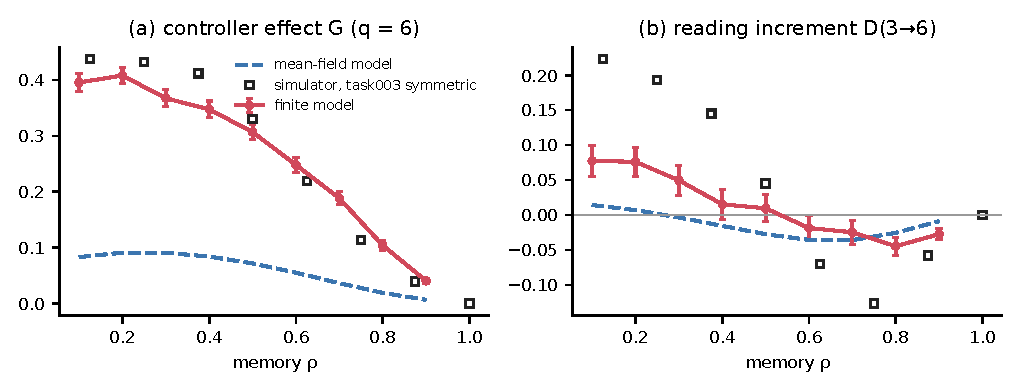
\includegraphics[width=\linewidth]{fig5_finite_reversal.pdf}
\caption{\textbf{Finite against mean-field model}, with the simulator (task003 symmetric) shown for reference only,
not fitted.}
\label{fig:finite}
\end{figure}
\begin{figure}[h]
\centering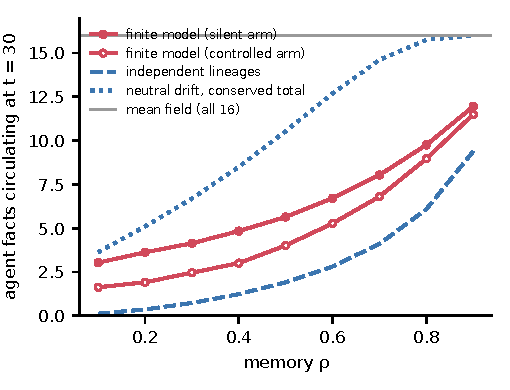
\includegraphics[width=0.5\linewidth]{fig6_diversity.pdf}
\caption{\textbf{Diversity collapse:} agent facts still circulating at $t=30$. Most die out at short memory. Two
analytic approximations built from mean-field quantities (independent two-type branching, and neutral drift at a
conserved total) bracket the finite model at every memory computed.}
\label{fig:div}
\end{figure}
\begin{figure}[h]
\centering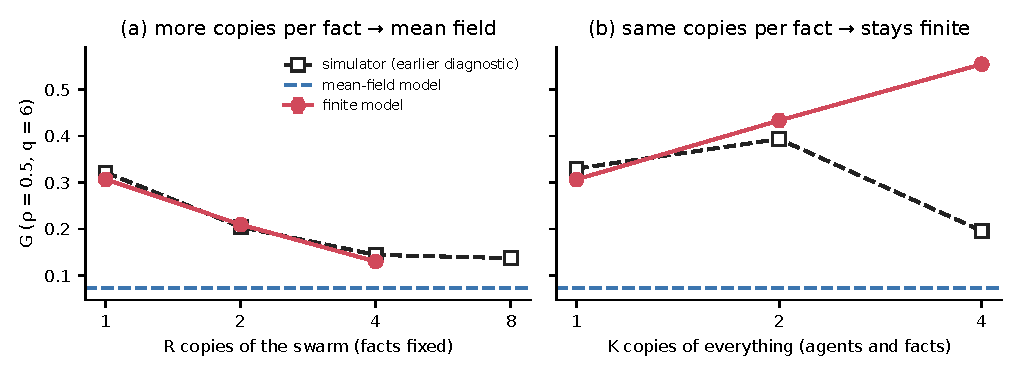
\includegraphics[width=\linewidth]{fig7_scaling.pdf}
\caption{\textbf{Scaling.} (a) More copies per fact (the swarm copied $R$ times, facts fixed) drives the effect to the
mean field, almost as in the simulator's earlier diagnostic. (b) Copying agents and facts together keeps copies per
fact, and the effect stays large. The simulator falls at $K=4$, where single facts are less informative, which the
model does not represent.}
\label{fig:scale}
\end{figure}

\begin{result}[finite size enlarges the controller]
At $\rho=0.1$ only 1.6 of 16 agent facts are still circulating at $t=30$; at $\rho=0.9$, 11.5 are. All four controller
facts survive. The controller effect rises from 0.07--0.09 (mean field) to 0.31--0.41, against 0.33--0.44 in the
simulator. The reversal remains, with its crossover at $\rho\approx0.5$--$0.6$ (simulator: 0.5--0.625). Removing the
controller's facts leaves lasting damage ($+0.036$; simulator $+0.04$). Copying the swarm gives $G=0.31,0.21,0.13$ for
$R=1,2,4$, against the simulator's $0.32,0.20,0.14$.
\end{result}
\paragraph{Why.} The controller recycles a few facts that survive, while the swarm's evidence is spread over many facts
that die out. Extinction thus removes the swarm's protection but not the controller's attack. In a control with the same
total controller evidence spread over 16 facts, the amplification over the mean field fell from $4.2\times$ to
$2.4\times$. My first run of that control kept the per-fact strength fixed instead, which changed the total evidence; the
error is logged. The effective finite size is \emph{copies per fact}, roughly $N/F$ and $W/F$, not $N$. Every agent fact
sits near its growth threshold ($\mathcal R_f\approx0.8$--$1.1$), so diversity is set by drift. The ChatGPT agent gave
the exact conserved-total version: equal mean copy numbers can hide very different surviving diversity.

\paragraph{Gating makes persistence fade.} With neutral reposting the finite model keeps 0.91--0.99 of its effect after
100 time units, like task003. With reposting tied to the vote ($\varepsilon=0.5$) it keeps 0.55 and 0.30, and is still
falling, like Object Placements (Fig.~\ref{fig:gate}). Controller lineages lose their reposters and go extinct one at a
time. This is finite-size selection, consistent with the earlier finding that persistence is shaped by the posting
rule's selection.
\begin{figure}[h]
\centering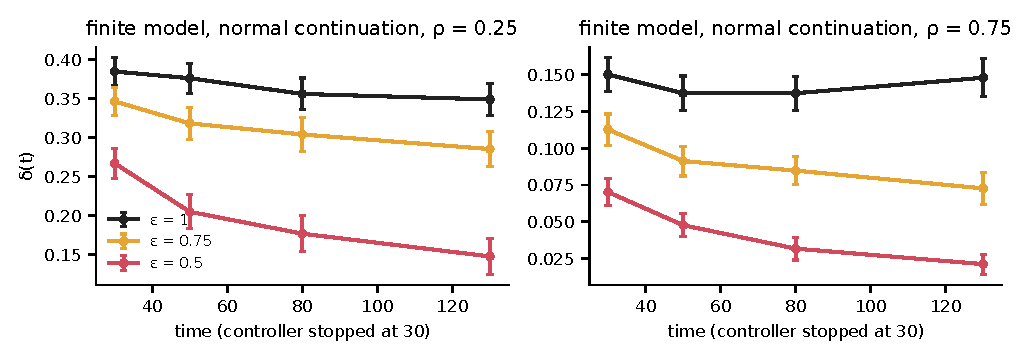
\includegraphics[width=\linewidth]{fig9_gating.pdf}
\caption{\textbf{Vote gating in the finite model} (normal continuation). Neutral reposting ($\varepsilon=1$) persists;
gated reposting fades over tens of time units.}
\label{fig:gate}
\end{figure}

% ======================================================================================================================
\section{Where the reversal happens: counter-evidence, not proofs}
Proofs do not move the crossover. Adding a proof variable, with sizes taken from the worlds and with exact co-retention
of a proof's facts, leaves the model's crossover unchanged. The simulator explains why: at its own crossovers only 1\%
(task003) and 3\% (Object Placements) of agents hold a complete proof.

Instead, the protective term of Eq.~\eqref{eq:rev} scales with $\beta_A$, how strongly the agents' own facts argue
against $A2$. We measured an effective $\beta_A$ in each setup from 72{,}000 stored memories, by a least-squares fit of the
exact $\operatorname{logit}P(A2\mid M)$ on the counts of facts held. No votes or effect sizes enter this measurement.
\begin{figure}[h]
\centering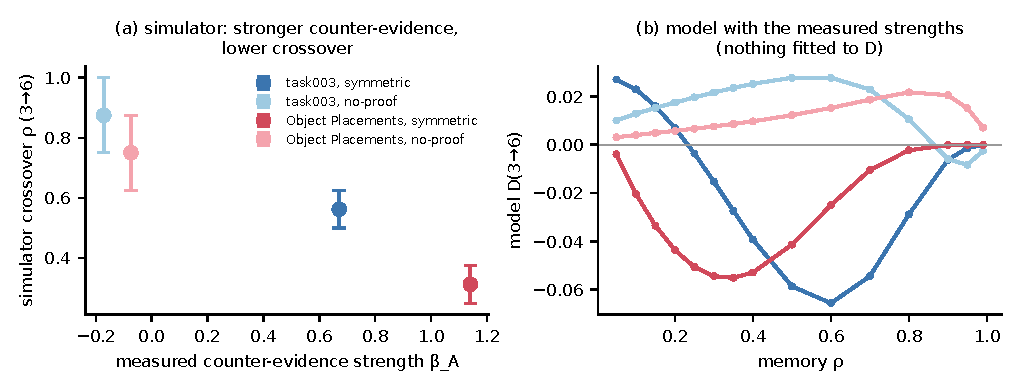
\includegraphics[width=\linewidth]{fig8_counterevidence.pdf}
\caption{\textbf{(a)} In the simulator, setups whose agents hold stronger counter-evidence reverse at shorter memory.
\textbf{(b)} The model with the measured strengths.}
\label{fig:ce}
\end{figure}
\begin{result}[counter-evidence orders the crossovers]
The measured $\beta_A$ values are 1.14 (Object Placements symmetric), 0.67 (task003 symmetric), $-0.07$ (Object
Placements no-proof) and $-0.17$ (task003 no-proof). This is exactly the reverse of the order of the simulator's
crossovers, as predicted in advance (Fig.~\ref{fig:ce}a). No-proof agents' facts do not argue against $A2$: together they
point to an even split. The model with the measured strengths reproduces the symmetric/no-proof contrast, but swaps the
two no-proof setups (Fig.~\ref{fig:ce}b).
\end{result}

% ======================================================================================================================
\section{What persuades: fact identity, context, and population susceptibility}\label{sec:persuade}
\paragraph{A deciding test.} Does the effect of adding one controller fact to a memory, $\Delta P=P(A2\mid M\cup f)-
P(A2\mid M)$, depend on how many agent facts are held (my count response) or on which combinations are held (the ChatGPT
agent's response)? Both predictions were fixed in advance, with episodes and reading conditions held out.
\begin{itemize}
\item \textbf{Both fail.} Held-out $R^2\approx0$ in all four setups.
\item \textbf{Post-hoc:} the identity of the controller fact explains $R^2=0.38$--$0.78$.
\item \textbf{The ChatGPT agent's stronger version} controls for both identities. Specific combinations then reduce the
  remaining error by 9--26\% in every setup, including no-proof.
\item \textbf{The same controller fact can push toward or away from $A2$} at equal counts. Exactly,
  $\Delta P=\sigma(x+\theta_f(M))-\sigma(x)$, where the log-likelihood ratio $\theta_f$ changes sign with context.
\end{itemize}
So persuasiveness is neither a fixed property of a fact nor a function of counts.

\paragraph{Population susceptibility.} We summarised this at the population level as the average effect of the
controller facts actually encountered,
\begin{equation}
S(t)=\mathbb E_{M\sim\mu(t)}\,\mathbb E_{f\sim w(t)}\big[\sigma(x(M)+\theta_f(M))-\sigma(x(M))\big],\label{eq:S_t}
\end{equation}
where $\mu(t)$ is the distribution of memories and $w(t)$ the mix of controller facts on the board. We measured it on
stored post-stop data (Fig.~\ref{fig:sus}).
\begin{figure}[h]
\centering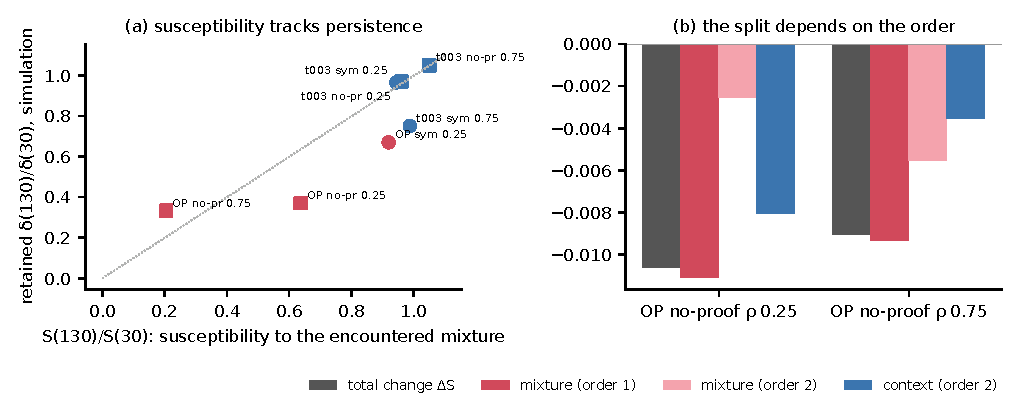
\includegraphics[width=\linewidth]{fig10_susceptibility.pdf}
\caption{\textbf{(a)} The change of population susceptibility from $t=30$ to 130 against the retained effect in the
simulation. \textbf{(b)} Splitting the change into ``mixture'' and ``context'' parts depends on the order of the split.}
\label{fig:sus}
\end{figure}
\begin{result}[susceptibility tracks persistence]
$S$ falls by 36\% and 80\% in Object Placements no-proof, where the effect fades, and stays within $\pm5\%$ in task003,
where it persists. It is not redundancy: a probe that removes already-held facts gives the same drops. Object Placements
symmetric is under-tracked: $-8\%$ against an effect that falls 33\%. Whether the drop comes from the changing mix of
facts or from the receivers' context cannot be decided, because the split depends on the order.
\end{result}

% ======================================================================================================================
\section{The ChatGPT agent's model and its assumptions}
\label{sec:gpt}
The ChatGPT agent built an independent engine-free model on the same day. Sources: its notes
\nolinkurl{2026-10-27_chatgpt_02}--\nolinkurl{_07} and its report
\nolinkurl{theory_chatgpt/reports/2026-10-27_phenomenological_model/}. Its guiding idea is different from mine:
\emph{a repeated, concentrated claim competes with information whose meaning needs to be put together}. Reading brings
in the controller's claim, but it also helps an agent gather the complementary facts that defuse it.

\paragraph{Ingredients.}
\begin{itemize}
\item $k$ interchangeable \emph{native} facts $A_1,\dots,A_k$ and \emph{one} introduced (controller) fact $C$. The board
  holds a share $b$ of $C$, and $(1-b)/k$ of each native fact.
\item Agents read $q$ posts drawn with replacement at rate 1 and forget each fact at rate $\gamma$.
\item The memory state keeps \emph{combinations}, not only single facts:
  \begin{itemize}
  \item $h_n$ is the probability of holding a given set of $n$ native facts;
  \item $j_n$ is the probability of holding $C$ together with such a set.
  \end{itemize}
  These follow exact ``co-retention'' equations: one read can bring in several facts at once, so remembered facts are
  correlated even though each is forgotten independently.
\item An \emph{assumed} all-or-nothing vote rule (Table~\ref{tab:gptrule}): single native facts do nothing; only the
  \emph{full} native set corrects.
\end{itemize}
\begin{table}[h]
\centering\small
\caption{\textbf{The ChatGPT agent's vote rule} for $k=6$: the probability of a wrong ($A2$) vote, by memory content.
These values are set by the rule, not computed by Bayes. ``Conclusive'' and ``inconclusive'' are its two versions,
meant loosely as analogues of our symmetric and no-proof setups.}
\label{tab:gptrule}
\begin{tabular}{@{}lrr@{}}\toprule
Memory contents & conclusive & inconclusive\\\midrule
nothing, or only part of the native set & 1/3 & 1/3\\
$C$, with none or only part of the native set & 2/3 & 2/3\\
full native set, without $C$ & 0 & 1/6\\
full native set, with $C$ & 0 & 1/4\\\bottomrule
\end{tabular}
\end{table}

\paragraph{Equations.} Averaging that rule over memories, and doing the same for posting, gives
\begin{align}
\Phi&=p_0-\beta\,\widetilde h_k+\alpha\,(\widetilde j_0-\eta\,\widetilde j_k),\label{eq:gptphi}\\
w_A&=k\kappa_A\widetilde h_1,\qquad w_C=\kappa_C(\widetilde j_0-\chi\,\widetilde j_k),\label{eq:gptpost}
\end{align}
where a tilde marks memory just after reading. $w_C$ says an agent reposts $C$ only if it does not hold the full native
set ($\chi=1$). Memory relaxes faster than the board, so the moments can be set to their stationary values at the
current $b$. Only \emph{two} variables then evolve, the board share of $C$ and the mean last vote $v$:
\begin{equation}
\dot b=\nu\{w_C(b)-b\,[w_A(b)+w_C(b)]\}+J(t)(1-b),\qquad \dot v=\Phi(b)-v.\label{eq:gpt2}
\end{equation}
Here $\nu=N/W$ and $J(t)$ is the controller's posting rate. The reduction matches the 15-variable version to within
$1.3\times10^{-4}$ in $G$.

\paragraph{What it showed.}
\begin{itemize}
\item \textbf{Reversal, only for large combinations.} With $k=6$ the reversal appears with fixed coefficients:
  $D(3\to6)=+0.036$ at $\rho=0.125$ and $-0.093$ at $\rho=0.875$, with the crossover between 0.25 and 0.5.
  With $k=2$ and $k=3$ it \emph{fails}. Since Object Placements' smallest proofs have three facts, $k$ cannot simply be
  read as proof size.
\item \textbf{Persistence as a self-sustaining information state.} After the stop, the model settles to a stable
  positive equilibrium (retained $G=0.093$ and $0.073$ at $\rho=0.25$, $0.75$). This happens because $C$ can invade the
  $C$-free state: its growth number is 1.27 and 1.59. No bistability is needed. This is the same kind of threshold as
  my Eq.~\eqref{eq:R}, derived independently.
\item \textbf{Prevalence is not persuasion.} At long memory, $C$ is held more often (0.34 against 0.13) yet persuades
  less.
\item \textbf{Exact frozen-board co-retention,} checked against eight stored simulator cells. Multiplying single-fact
  probabilities underestimates how often whole combinations are held.
\item \textbf{Exact finite-size results} (Section~\ref{sec:div}): for independent lineages and for bounded neutral
  copying (a Moran process, in which each new copy replaces an old one), the mean number of copies is conserved while
  the surviving diversity collapses.
\item \textbf{Held-out response tests}
  (Section~\ref{sec:persuade}): context matters in all four setups, but the all-or-nothing rule is \emph{not}
  supported.
\end{itemize}

\section{The two approaches compared}
\begin{table}[h]
\centering\footnotesize
\caption{\textbf{Assumptions and results of the two models, side by side.} The fact-flow model is that of
Sections~2--5; the combination toy is that of Section~\ref{sec:gpt}.}
\label{tab:compare}
\begin{tabular}{@{}p{0.17\linewidth}p{0.385\linewidth}p{0.385\linewidth}@{}}\toprule
 & \textbf{Fact flow (Claude)} & \textbf{Combination toy (ChatGPT)}\\\midrule
Controller facts & $F_C=4$ interchangeable facts & one fact $C$\\[2pt]
Native facts & $F_A=16$, each a small graded piece of counter-evidence & $k=6$, individually inert\\[2pt]
Evidence response & smooth sigmoid of counts, Eq.~\eqref{eq:phi} & all-or-nothing on the full set, Eq.~\eqref{eq:gptphi}\\[2pt]
Memory & per-fact averages (independent facts) & exact co-retention of combinations\\[2pt]
Reposting & proportional to memory, optional vote gating $\varepsilon$ & memory-based; $C$ not reposted once fully corrected\\[2pt]
Finite size & explicit finite version; facts can die out & deterministic only (exact lineage results separate)\\[2pt]
Reversal mechanism & displacement against flattening sensitivity, Eq.~\eqref{eq:rev} & reading assembles the corrective combination\\[2pt]
Persistence mechanism & growth number $\mathcal R_C>1$; finite gating gives fading & invasion of the $C$-free state; stable positive equilibrium\\[2pt]
Reversal holds for & 16 of 22 parameter changes; $F_C=F_A$ too & $k=6$ only; fails for $k=2,3$\\[2pt]
Effect size & mean field 3--10$\times$ too small; finite model at simulator level & comparable to mean field (0.07--0.09)\\[2pt]
Main weakness & counts miss which fact and in which context ($R^2\approx0$) & all-or-nothing rule not supported; no diversity loss\\\bottomrule
\end{tabular}
\end{table}
Table~\ref{tab:compare} sets out the differences. Three points matter most.
\begin{enumerate}
\item \textbf{Both explain the reversal as a competition inside reading,} but between different things. In mine, reading
  pushes the controller's displacement up and the agents' sensitivity down. In ChatGPT's, reading brings in $C$ but also
  completes the correction. The deciding test of Section~\ref{sec:persuade} rejected both pure forms: neither counts nor
  combinations predict persuasion.
\item \textbf{Both find the same persistence threshold:} information keeps circulating when one copy produces more than
  one copy before it is lost. This independent agreement is the most solid shared result.
\item \textbf{Only my model has finite size,} and only finite size gives the effect at the simulator's size, lasting
  damage, and slow fading. Only ChatGPT's model has exact co-retention, which my count model averages away. ChatGPT's
  own report judged the finite fact-flow model to be ``the stronger baseline'' and its co-retention the most useful
  addition.
\end{enumerate}

\section{The model we are converging on, and why}
\begin{figure}[h]
\centering
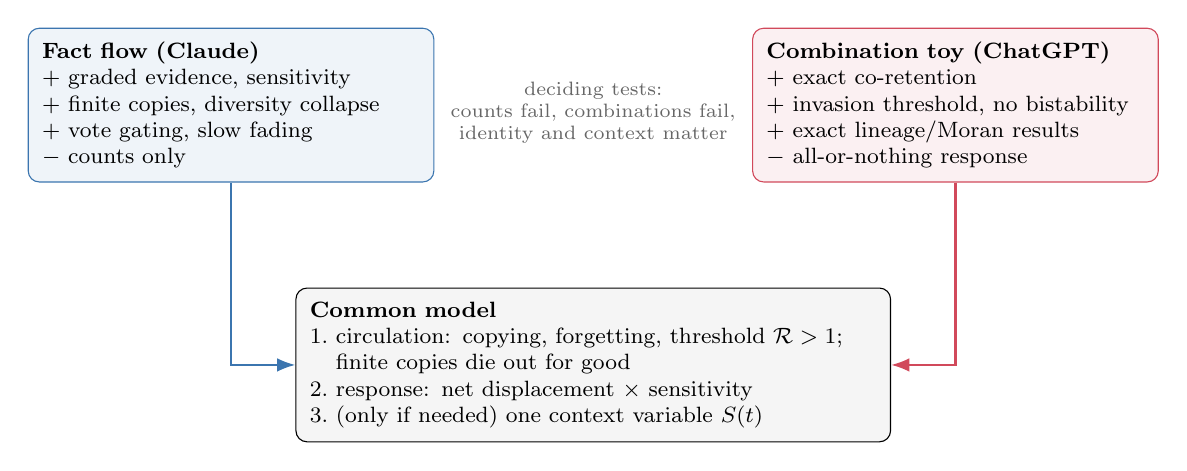
\begin{tikzpicture}[font=\small, >=Latex,
  box/.style={draw, rounded corners, align=left, inner sep=5pt, text width=48mm, font=\footnotesize}]
  \node[box, draw=cA, fill=cA!8] (cl) at (-4.6,0) {\textbf{Fact flow (Claude)}\\ $+$ graded evidence, sensitivity\\
    $+$ finite copies, diversity collapse\\ $+$ vote gating, slow fading\\ $-$ counts only};
  \node[box, draw=cC, fill=cC!8] (gp) at (4.6,0) {\textbf{Combination toy (ChatGPT)}\\ $+$ exact co-retention\\
    $+$ invasion threshold, no bistability\\ $+$ exact lineage/Moran results\\ $-$ all-or-nothing response};
  \node[box, draw=black, fill=black!4, text width=72mm] (cm) at (0,-3.3) {\textbf{Common model}\\
    1.\ circulation: copying, forgetting, threshold $\mathcal R>1$;\\ \phantom{1.\ }finite copies die out for good\\
    2.\ response: net displacement $\times$ sensitivity\\
    3.\ (only if needed) one context variable $S(t)$};
  \node[font=\scriptsize, align=center, text=black!60] (t) at (0,-0.1) {deciding tests:\\ counts fail, combinations fail,\\ identity and context matter};
  \draw[->, thick, cA] (cl.south) |- (cm.west);
  \draw[->, thick, cC] (gp.south) |- (cm.east);
\end{tikzpicture}
\caption{\textbf{What each model brought to the common model.} The held-out tests decided which parts survive.}
\label{fig:converge}
\end{figure}
Written as equations, the common model has three layers (Fig.~\ref{fig:converge}). They are the levels of the
hierarchy the ChatGPT agent proposed and I accepted.
\begin{enumerate}
\item \textbf{Circulation} (exposure). The copies of each fact on the board and in memories follow copying and
  forgetting, Eqs.~\eqref{eq:m}--\eqref{eq:b}. A class keeps circulating after the stop if its growth number exceeds one,
  Eq.~\eqref{eq:R}. In a finite swarm each fact's copy number can hit zero, which is permanent.
\item \textbf{Response.} The wrong-vote probability is a sigmoid of net evidence,
  \begin{equation}
  \Phi_2=\sigma\big(x_s+B\big),\qquad B=\bar\theta_C(t)\,M_C-\beta_A\big(M_A^{C}-M_A^{S}\big),\label{eq:common}
  \end{equation}
  so that $G=\sigma(x_s+B)-\sigma(x_s)$. The reversal is the competition of Eq.~\eqref{eq:rev}.
\item \textbf{Context, only if needed.} The fixed controller strength $\beta_C$ is replaced by $\bar\theta_C(t)$, the
  mean persuasive strength of the controller facts actually encountered, in their current contexts. It is measured by
  the susceptibility $S(t)$ of Eq.~\eqref{eq:S_t}. In task003 it is roughly constant, and the model reduces to my
  count model. In Object Placements it falls, and the effect fades even while the facts still circulate.
\end{enumerate}

\paragraph{Why this model, and not either of ours.}
\begin{itemize}
\item \textbf{The circulation layer} is common ground. Both of us derived the same growth threshold independently.
\item \textbf{The sigmoid response} stays because the reversal needs no proof:
  \begin{itemize}
  \item it holds in no-proof setups;
  \item completed proofs are rare at the crossover (1--3\%);
  \item the all-or-nothing rule works only for one chosen $k$ and fails at $k=3$.
  \end{itemize}
  ChatGPT gave up its conjunction as the default for these reasons.
\item \textbf{Counts alone are not enough:} they predict nothing in held-out data, and the same fact can push either
  way. I gave up the count model as a complete description of persuasion.
\item \textbf{Combinations alone are not enough either.} Once identities are controlled for, joint terms add only
  9--26\%. So we keep one coarse context variable instead of a catalogue of combinations. The ChatGPT agent insisted on
  this, so as not to import the simulator's likelihood tables into the theory.
\item \textbf{Finite diversity loss} is needed for the effect's size, lasting damage and slow fading. ChatGPT's exact
  Moran result shows why mean-field copy counts cannot capture it.
\end{itemize}

\paragraph{What is not yet agreed.} The framework is shared; a validated state equation for layer 3 is not. Open
questions:
\begin{itemize}
\item \textbf{The dynamics of $\bar\theta_C(t)$.} How it should evolve is open, and so is whether a small mixture of
  fixed strengths could stand in for it. Fixed strengths cannot reproduce the sign changes, but they might still suffice
  for the two population phenomena.
\item \textbf{Rare proof holders.} The ChatGPT agent cautions that they may still matter through what they later post.
  Only an intervention could rule this out.
\end{itemize}
Each agent also corrected the other on the way:
\begin{itemize}
\item net displacement instead of dose;
\item an observed bracket, not a proven bound;
\item persistence without bistability;
\item withdrawing my claim that additive evidence cannot combine constant circulation with falling persuasion;
\item an audit showing my board-window shortcut misses fewer than 0.01 facts.
\end{itemize}

\section{Limitations and next steps}
\begin{itemize}
\item \textbf{Not explained:}
  \begin{itemize}
  \item the size of $D$ (2--3 times too small in the finite model);
  \item the $K$-projects scaling at $K=4$;
  \item the order of the two no-proof setups;
  \item the under-tracked Object Placements symmetric persistence.
  \end{itemize}
\item \textbf{Closed forms not obtained:} the crossover position $\rho^*(q)$, and the number of surviving facts (only
  bracketed).
\item \textbf{The central open problem:} a compact law for how $S(t)$ evolves. Why does it fall in Object Placements and
  not in task003? A candidate: support-based reposting keeps recirculating controller facts that persuade only in
  contexts that are disappearing.
\item \textbf{Next:} write and test a small dynamical equation for $S(t)$ jointly with the ChatGPT agent, pre-registered,
  engine-free and judged qualitatively. Derive $\rho^*(q)$ from Eq.~\eqref{eq:rev}.
\end{itemize}

\paragraph{Reproducibility.} Model and runs: \nolinkurl{analysis/theory_claude/phenomenological_fact_flow/}, whose
decision log records every pre-registration and failure. Tests: \nolinkurl{discriminating_test/} and
\nolinkurl{mixture_probe/}. Exchange with the ChatGPT agent: \nolinkurl{analysis/theory_blackboard/}. Earlier reports of
this session: \nolinkurl{reports/2026-10-27_fact_flow_model/} and \nolinkurl{2026-10-28_*}.

\end{document}
